\documentclass{article}

% if you need to pass options to natbib, use, e.g.:
% \PassOptionsToPackage{numbers, compress}{natbib}
% before loading nips_2017
%
% to avoid loading the natbib package, add option nonatbib:
% \usepackage[nonatbib]{nips_2017}

\usepackage{nips_2017}

% to compile a camera-ready version, add the [final] option, e.g.:
% \usepackage[final]{nips_2017}
\usepackage[pdftex]{graphicx}
\usepackage[utf8]{inputenc} % allow utf-8 input
\usepackage[T1]{fontenc}    % use 8-bit T1 fonts
\usepackage{hyperref}       % hyperlinks
\usepackage{url}            % simple URL typesetting
\usepackage{booktabs}       % professional-quality tables
\usepackage{amsfonts}       % blackboard math symbols
\usepackage{nicefrac}       % compact symbols for 1/2, etc.
\usepackage{microtype}      % microtypography

\title{ML Project: Minist handwritten-digits recognition}

% The \author macro works with any number of authors. There are two
% commands used to separate the names and addresses of multiple
% authors: \And and \AND.
%
% Using \And between authors leaves it to LaTeX to determine where to
% break the lines. Using \AND forces a line break at that point. So,
% if LaTeX puts 3 of 4 authors names on the first line, and the last
% on the second line, try using \AND instead of \And before the third
% author name.

\author{
  	Qiming Zheng \\
	Shanghai Jiao Tong University\\
	\texttt {zqmmqz@sjtu.edu.cn}\\
	\And
	Shenggan Cheng \\
 	Shanghai Jiao Tong University\\
      \texttt {csg@sjtu.edu.cn}\\
}

\begin{document}
% \nipsfinalcopy is no longer used

\maketitle

\begin{abstract}

In this task, we investigate the mainstream techniques used in hand-written digit recognition task.
The dataset given for this project is based on Mixed National Institute of Standards and Technology database (MNIST) and this project aims to explore how computer can recognizes digits from images. Given pixel value vectors as features, we leveraging four classification models to predict the label of images. The models are softmax regression, support vector machine (SVM), k-nearest neighbors(k-NN) and convolutional neural network (CNN). This work we engaged in can be applied in image recognition and classification for handwriting digit, which is a significant topic in machine learning field.

\end{abstract}

\section{Dataset Exploration}


The dataset used in this task comes from MNIST hand-written digits libraies. The dataset is composed of 70000 samples totally. The digits classes distribution of samples is balanced (Figure~\ref{data_dist}), each sample image has a width and height at 45 pixels. The test dataset has 10000 samples.

I pick 5000 images from the 60000 training samples as the validation sets to avoid overfitting(especially in deep learning models).

The handwritten digits are collected from  Census Bureau employees and  high-school students. The clearness of the digits from employess are much cleaner than that of high-school students. Thus easier to recognize.

Each image is composed of 45x45 pixels and the pixel values range from 0 to 255. For the convenience of some algorithms (in terms of input data shape), the images need to be flattened to be a vector $\vec x = (x_1,x_2...x_d)^T$ (d=45x45). 

\begin{figure}[!h]
\centering
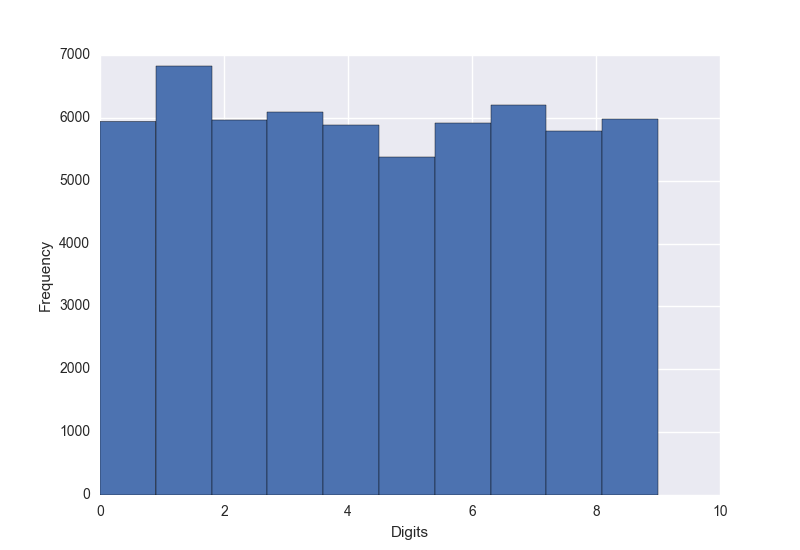
\includegraphics[width=3.5in]{image/train_data_dist}
\caption{The distribution of digits in training set}
\label{data_dist}
\end{figure}

\begin{figure}[!h]
\centering
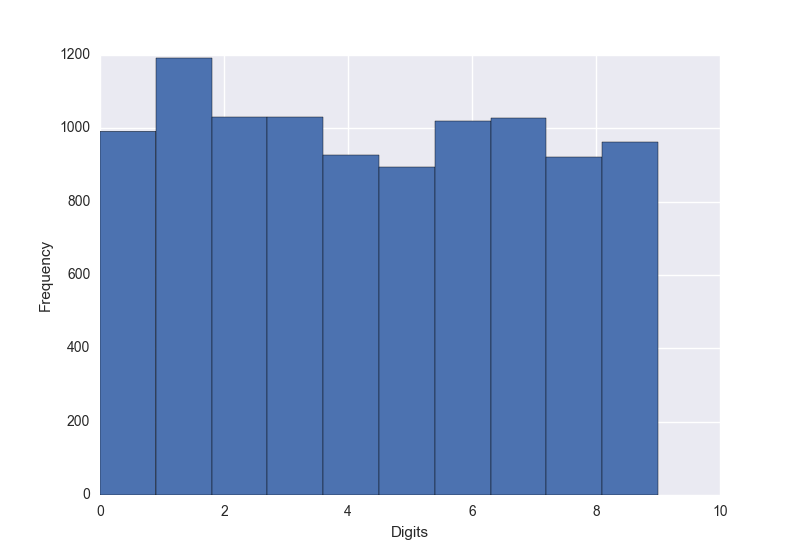
\includegraphics[width=3.5in]{image/test_data_dist}
\caption{The distribution of digits in test set}
\label{data_dist}
\end{figure}


\subsection{Task Description}

Our task is to recognize a Arabic numeral from an image. The prediction process includ the following three steps. First we read in and preprocess the nxn pixels square images with an handwritten digit on it (in our case the image is 28x28 pixels). Each pixel on the image was convert into a number between 0 and 1, with 0 as black and 1 as white. It was then saved in a vector denoted as $\vec x = (x_1, x_2, ..., x_{n^2} )$. The label of each image was saved in a one-hot encoding which we denoted as y = (y0, y1, ..., y9). 

For example, (0, 0, 0, 0, 0, 1, 0, 0, 0, 0) represents a label of 5. Then we train different classification models with the training set of the data. After training, for each image in the test set, the classifiers returned a normalized probability for each class and the class with the highest probability is chosen to represent the image. Eventually, the accuracy was calculated by dividing the number of correct prediction made by the classifier with the the total number of prediction made. The classification models applying here are discribe in detail in section 3.

To measure the performance of the model I chosed, a baseline model I used is a simple cosine similarity model. An mean image for each Arabic numeral in the training set is calculated as given in part 1. Then for each image in test set, we calculated the cosine similarities with the mean images. The image was classified to one of Arabic numerals according to the highest cosine similarity. This simple model is 82.21$\%$ accurate.

In fact, the process of the learning algorithm is quite slow for the high dimension of sample images. Thus, in addition to the original data processing method, we also
used a dimensional reduction method named principal component analysis (PCA) to reduce the computational cost. Detail of the PCA and the comparisons of each model with and without PCA are discribed later.

\subsection{Dimension Reduction}


For the constraint of computational resources, I have to first reduce the dimension of the data points from a 45x45 images to a less resolutionary one.

This step is conducted through PCA: a popular statistical procedure that uses the orthogonal linear transformation to convert a set of data to a new feature space such that the greatest variance by the projection of the data comes to lie on the first coordinate (called the first principal component), the second greatest variance on the second coordinate, and so on.

The primal components should maximize the covariance of the original vectors $X = [\vec x_1, \vec x_2, ...\vec x_m]$ under new basis:
\begin{equation}
max tr(W^T X X^T W)
\end{equation}
\[
s.t. W^t W=I
\]

where the W form the new basis of the reduction space. Using Lagrangian method to solve this convex optimization problem:
\begin{equation}
X X^T w_i = \lambda_i w_i
\end{equation}

It’s obvious that the k largest eigenvalues and the corresponding eigenvectors form the basis. To quantify the reduction extend, we can use the weight of the chosen eigenvalues compared with all the eigenvalues as the notification. That is to say: the reduced data can approximate the
original data by a factor of : 

\begin{equation}
\rho = \frac{\sum_{i=1}^{k} \lambda_i}{\sum_{i=1}^{k} \lambda_j}
\end{equation}

A scattering of the dimension reduction result can be seen in Figure~\ref{PCA}.

\begin{figure}[!h]
\centering
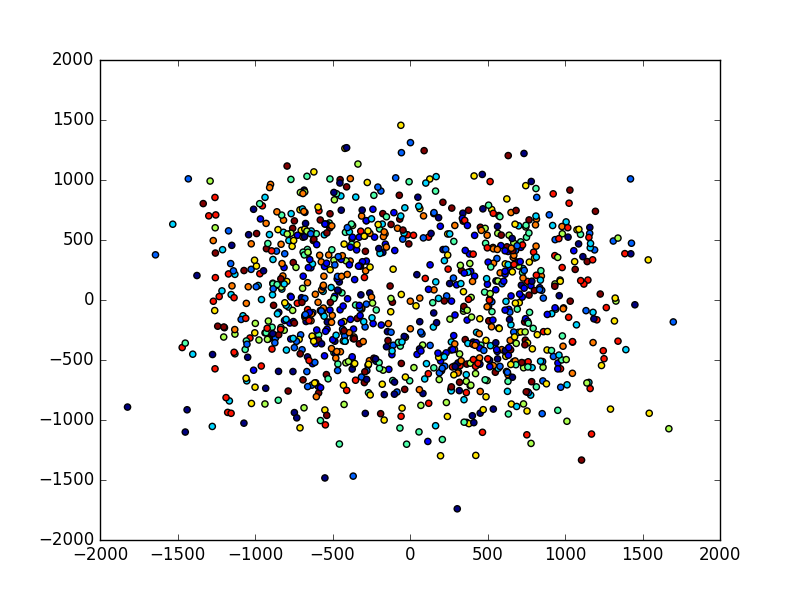
\includegraphics[width=4.5in]{image/pca_scatter}
\caption{PCA visualization 1}
\label{PCA}
\end{figure}

The explained portion of different used principal component is shown in Figure~\ref{PCA2}

\begin{figure}[!h]
\centering
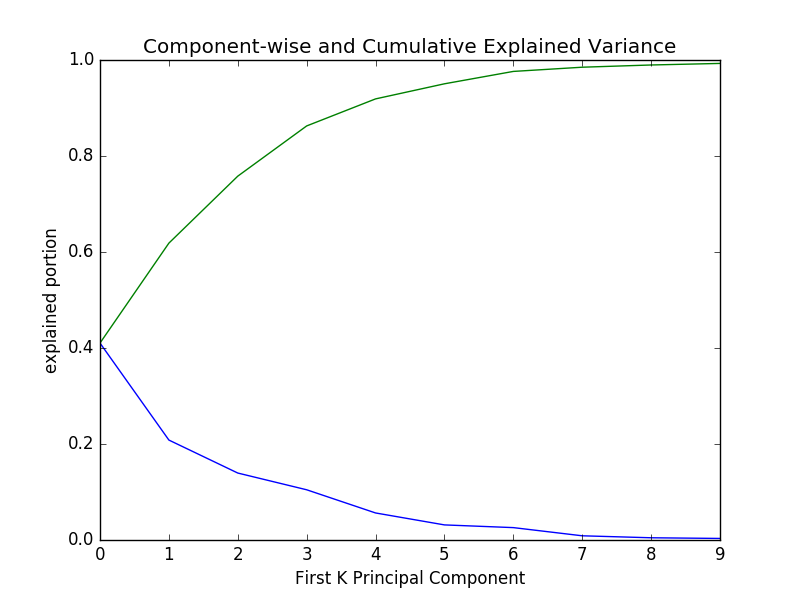
\includegraphics[width=4.5in]{image/pca_curve}
\caption{PCA visualization 2}
\label{PCA2}
\end{figure}

\section{Machine Learning Models}
\subsection{Softmax Regression}

Softmax regression is a multiple class version of logistic regression.
In logistic regression, the labels are restricted to 0 and 1, which output a classification of two classes. (i.e. $y^i \in \{0,1\}$. However, softmax regression allows us to handle multiple classes label outputs, by introducing a vector of sigmoid functions, which represents the probability of each label outputs.

The hypothesis equation goes like this: 
\begin{equation}
\sigma(x) = \left[
 \begin{matrix}
   P(y=0|x;\theta)\\
  P(y=1|x;\theta)\\
  ...\\
   P(y=9|x;\theta)
  \end{matrix}
  \right]
  =\frac{1}{\sum_0^9 exp(\theta^{(i)}x)}
  =\left[
 \begin{matrix}
  exp(\theta^{(0)}x)\\
  exp(\theta^{(1)}x)\\
  ...\\
  exp(\theta^{(9)}x)
  \end{matrix}
  \right]
\end{equation}

The wieght $\theta$ is determined by optimize the cross-entropy cost function:

\begin{equation}
arg min_{\theta}  -\sum_{i=0}^{m} \sum_{k=0}^{9} \sigma\{y^{(i)}=k\} log( \sigma_{y^{(i)}=k} (x) ) 
\end{equation}

By applying gradient descent method, we reached the minimum
of cost function and accordingly achieved a set of
model weights $\theta$.

\subsection{K-Nearset Neighbors}

The k-nearest neighbors algorithm (k-NN) is one of the non-parametric methods used for classification. The idea of k-NN is straight forward. In k-NN classification, an object is classified by a majority vote of its neighbors, with the object being assigned to the class most common among its k nearest neighbors (k is a positive integer, typically small)[1]. The simplest case is when k = 1, the test data is assigned to the class of that single nearest neighbor.

The choice of k is very critical for k-NN. A small value of k means that noise will have a higher influence on the result, while a large value of k can make boundaries between classes less distinct.

In this project, since the data are in 784 dimensional space, the computational cost is relatively high. It is sensible to pick a small k value. we run the algorithm for k from 1 to 10 and compute the classification accuracy on the validation dataset.

\subsection{Support Vector Machine}

Support vector machine (SVM) is originaly formulated for binary classification. SVM predict the points' belongings by finding a hyper-plane that seperate the datasets into different half-space. There were many hyperplanes that might classify the data. The hyperplane it chose represented the largest separation, or margin, between the two classes.

Intendented to seperate multiple classifications, SVM need to be extended into 1v1 or 1vAll versions of SVM.

Considering that the linear kernels can reach a relatively high prediction accuracy, and the high computation expenditure, I just tried the linear SVM as examples.

\textbf{Acceleration}

Considering the dataset size as well as the computation complexityof SVM($O(N^2)$), it's highly unreliable to run a sequential version of SVM on my machine, therefore, I use a multithread version SVM to accelarate the training processm the training speed has witnessed a giant leap.


\section{Deep Learning Models }


\section{Experiments}

\subsection{SVM}

The relation between dataset size and SVM classifier accuracy is shown in Figure~\ref{svm_curve}

\begin{figure}[!h]
\centering
\includegraphics[width=6.0in]{image/svm_curve}
\caption{SVM accuracy vs. training set size }
\label{svm_curve}
\end{figure}

\subsection{KNN}

The relation between dataset size and KNN classifier accuracy is shown in Figure~\ref{KNN_curve}

\begin{figure}[!h]
\centering
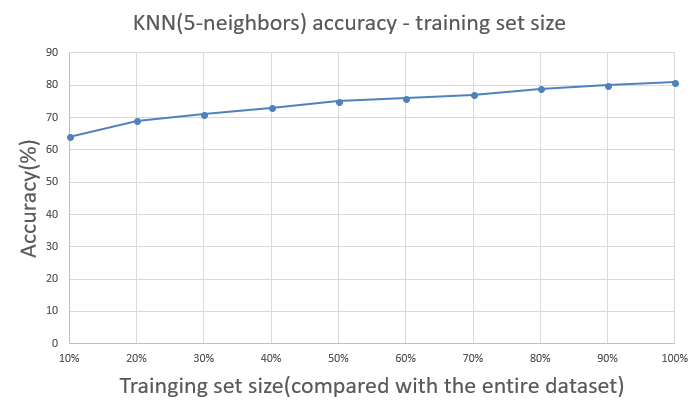
\includegraphics[width=6.0in]{image/KNN_curve}
\caption{KNN accuracy vs. training set size }
\label{KNN_curve}
\end{figure}

In this experiment, we fix the number of neigbors (K) to 5, actually, this number vary from 1 to 10 influence little to the final result, while a larger number neighbors cause great computation cost in the K-D tree building stage.

\section{Conclusion}


\section*{References}

References follow the acknowledgments. Use unnumbered first-level
heading for the references. Any choice of citation style is acceptable
as long as you are consistent. It is permissible to reduce the font
size to \verb+small+ (9 point) when listing the references. {\bf
  Remember that you can go over 8 pages as long as the subsequent ones contain
  \emph{only} cited references.}
\medskip

\small

[1] Alexander, J.A.\ \& Mozer, M.C.\ (1995) Template-based algorithms
for connectionist rule extraction. In G.\ Tesauro, D.S.\ Touretzky and
T.K.\ Leen (eds.), {\it Advances in Neural Information Processing
  Systems 7}, pp.\ 609--616. Cambridge, MA: MIT Press.

[2] Bower, J.M.\ \& Beeman, D.\ (1995) {\it The Book of GENESIS:
  Exploring Realistic Neural Models with the GEneral NEural SImulation
  System.}  New York: TELOS/Springer--Verlag.

[3] Hasselmo, M.E., Schnell, E.\ \& Barkai, E.\ (1995) Dynamics of
learning and recall at excitatory recurrent synapses and cholinergic
modulation in rat hippocampal region CA3. {\it Journal of
  Neuroscience} {\bf 15}(7):5249-5262.

\end{document}
